\documentclass[16pt,a4paper]{article}
\usepackage{graphicx} % Required for inserting images
\graphicspath{ {./images/} }

\begin{document}
\begin{titlepage}
    \begin{center}
        \vspace*{1cm}
        
        \Huge
        \textbf{Assignment 4}
        
        \vspace{0.5cm}
        \LARGE
        Ideal Gas Laws % comment out if irrelevant
        
        \vspace{1.5cm}
        
        \textbf{CH22B098-Samridhi Srivastava}
   		  \vspace{1.5cm}
        
        \textbf{Github ID- Samridhi24}
       
        \vfill
        
        
        
        \vspace{0.8cm}
          \Large
	    ID2090\\
          Department of Chemical Engineering,\\
        Indian Institute of Technology, Madras\\
        June 2023
        
    \end{center}
\end{titlepage}








\section{Ideal Gases}
The concept of ideal gases is useful for understanding gas behavior. It is also useful for simplification and calculation of gas properties.


For a gas to be ideal, there are four main assumptions to be made ~\cite{doi:10.1021/ed045p351.1}
\begin{itemize}
    \item The gas molecules have negligible volume
    \item The gas particles are equally sized. They neither attract nor repel each other, i.e, they have no inter-molecular forces.
    \item The gas particles move in a random, straight-line motion, in agreement with Newton's Laws of Motion
    \item The gas particles collide elastically with the walls of the container and with each other. There is no energy loss 
\end{itemize}



\section {Gas Laws}
\subsection{Boyle's Law}
In 1662, Boyle discovered that the relationship between Pressure(P) and Volume(V), assuming Temperature(T) and amount of gas(n) remains constant.

It is given by
\begin{equation}
    P \propto \frac{1}{V}
\end{equation}

\subsection{Charles' Law}
In 1787, French physicist Jacques Charles discovered that the relationship between Temperature(T) and Volume(V), assuming Pressure(P) and amount of gas(n) remains constant.

It is given by
\begin{equation}
    V \propto T
\end{equation}

\subsection{Avogadro's Law}
In 1811, Amedeo Avagadro discovered that the relationship between Amount of gas(n) and Volume(V), assuming Pressure(P) and Temperature(T) remains constant.

It is given by
\begin{equation}
    V \propto n
\end{equation}

\section {Ideal Gas Law}
The ideal gas law is the combination of of the three simple Gas Laws.


On combining the three equations we get:
\begin{equation}
    V \propto \frac{nT}{P}
\end{equation}


On replacing the proportionality sign we get the Ideal Gas Law:~\cite{doi:10.1021/ed062p399.1}
\begin{equation}
   PV=nRT
\label{eq:idealgaslaw}
\end{equation}
where,
\begin{itemize}
    \item P = Pressure,
    \item V = Volume,
    \item n = Amount of gas, i.e, number of moles,
    \item R = Universal Gas Constant,
    \item T = Absolute Temperature
\end{itemize}


In eq~\ref{eq:idealgaslaw}, the temperature value should be in absolute units so that the right hand side of eq~\ref{eq:idealgaslaw} does not become zero.


\subsection{Universal Gas Constant}
R has different values and units and its value can be found in online databases. Figure ~\ref{fig:figure1}, Figure~\ref{fig:figure2} and Figure~\ref{fig:figure3} present different values of R for various units of P, V, n and T. They are based on the values reported by Moldover \emph{et al.}~\cite{PhysRevLett.60.249} Their value was determined from measurements of the speed of sound in argon as a function of pressure at the temperature of the triple point of water.
\begin{figure}[!hbpt]
    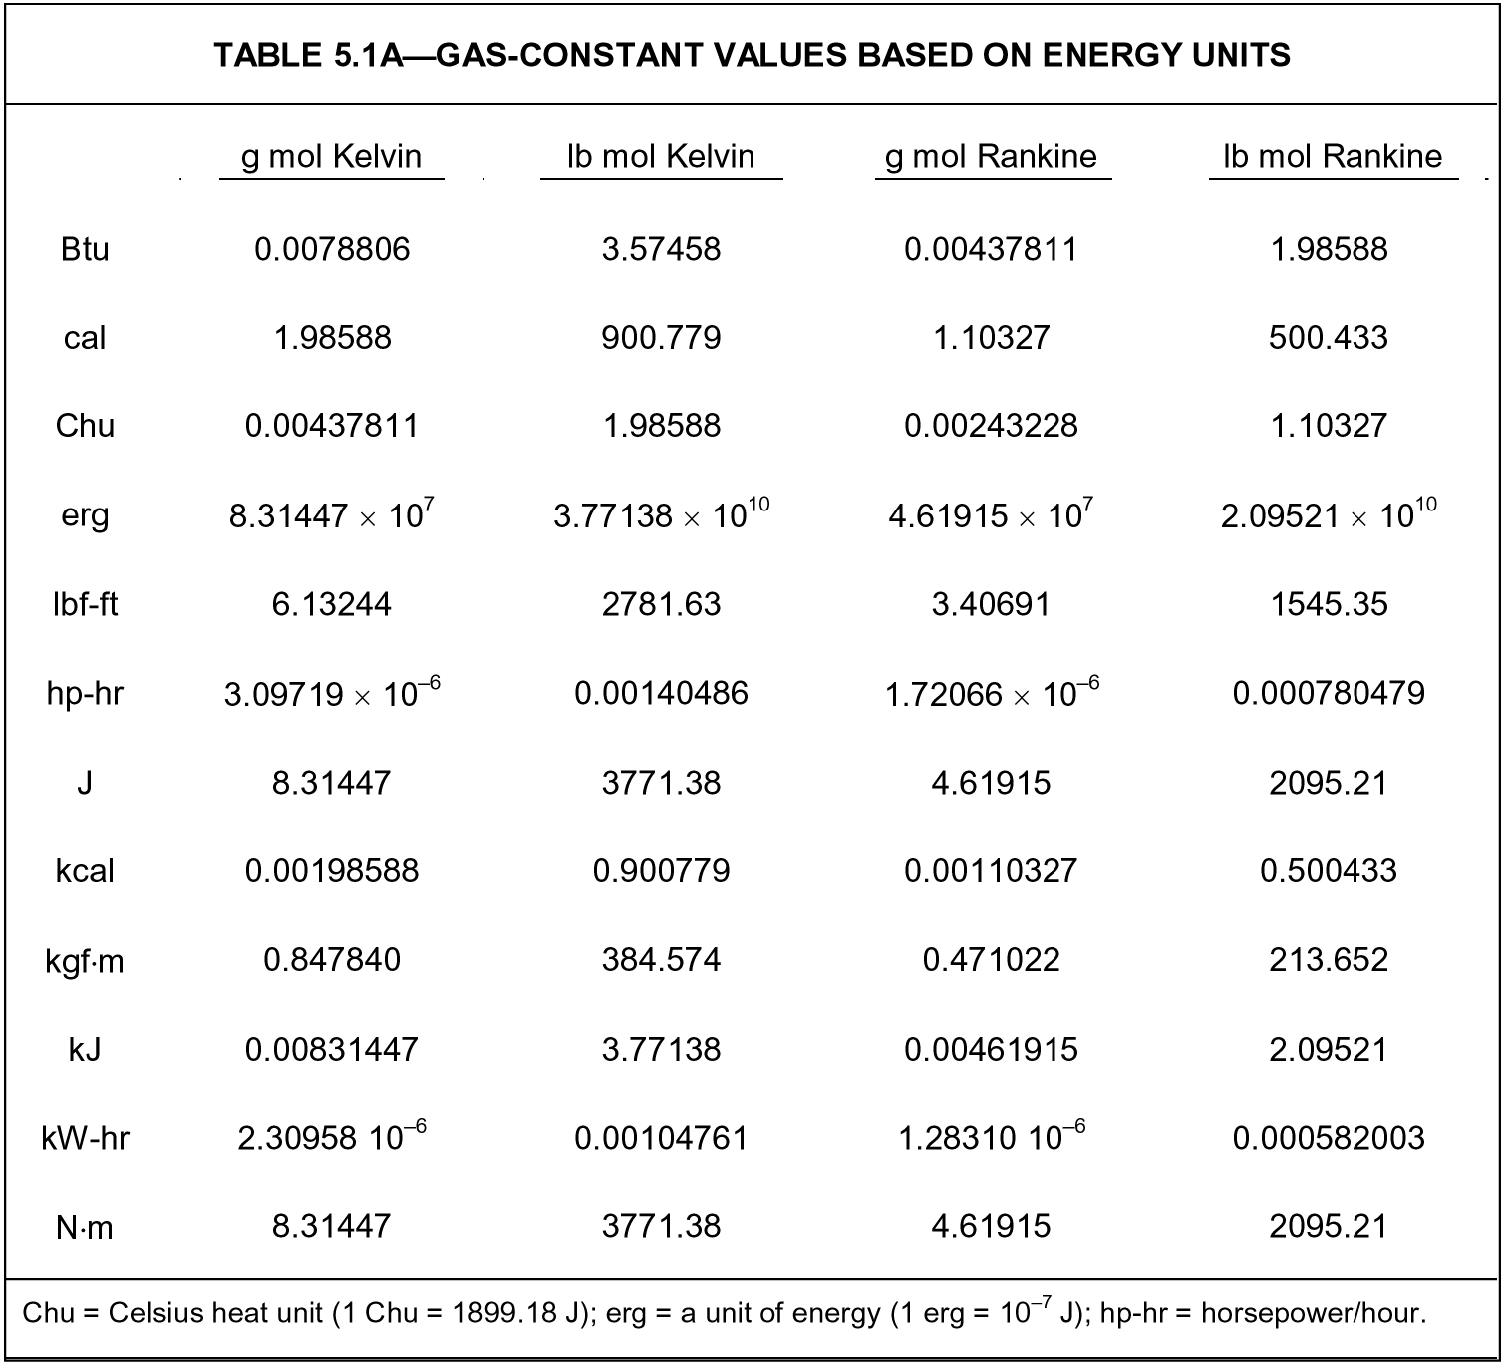
\includegraphics[scale=1]{images/vol_1.png}
    \caption{Table 1A}
    \label{fig:figure1}
\end{figure}
\begin{figure}[!hbpt]
    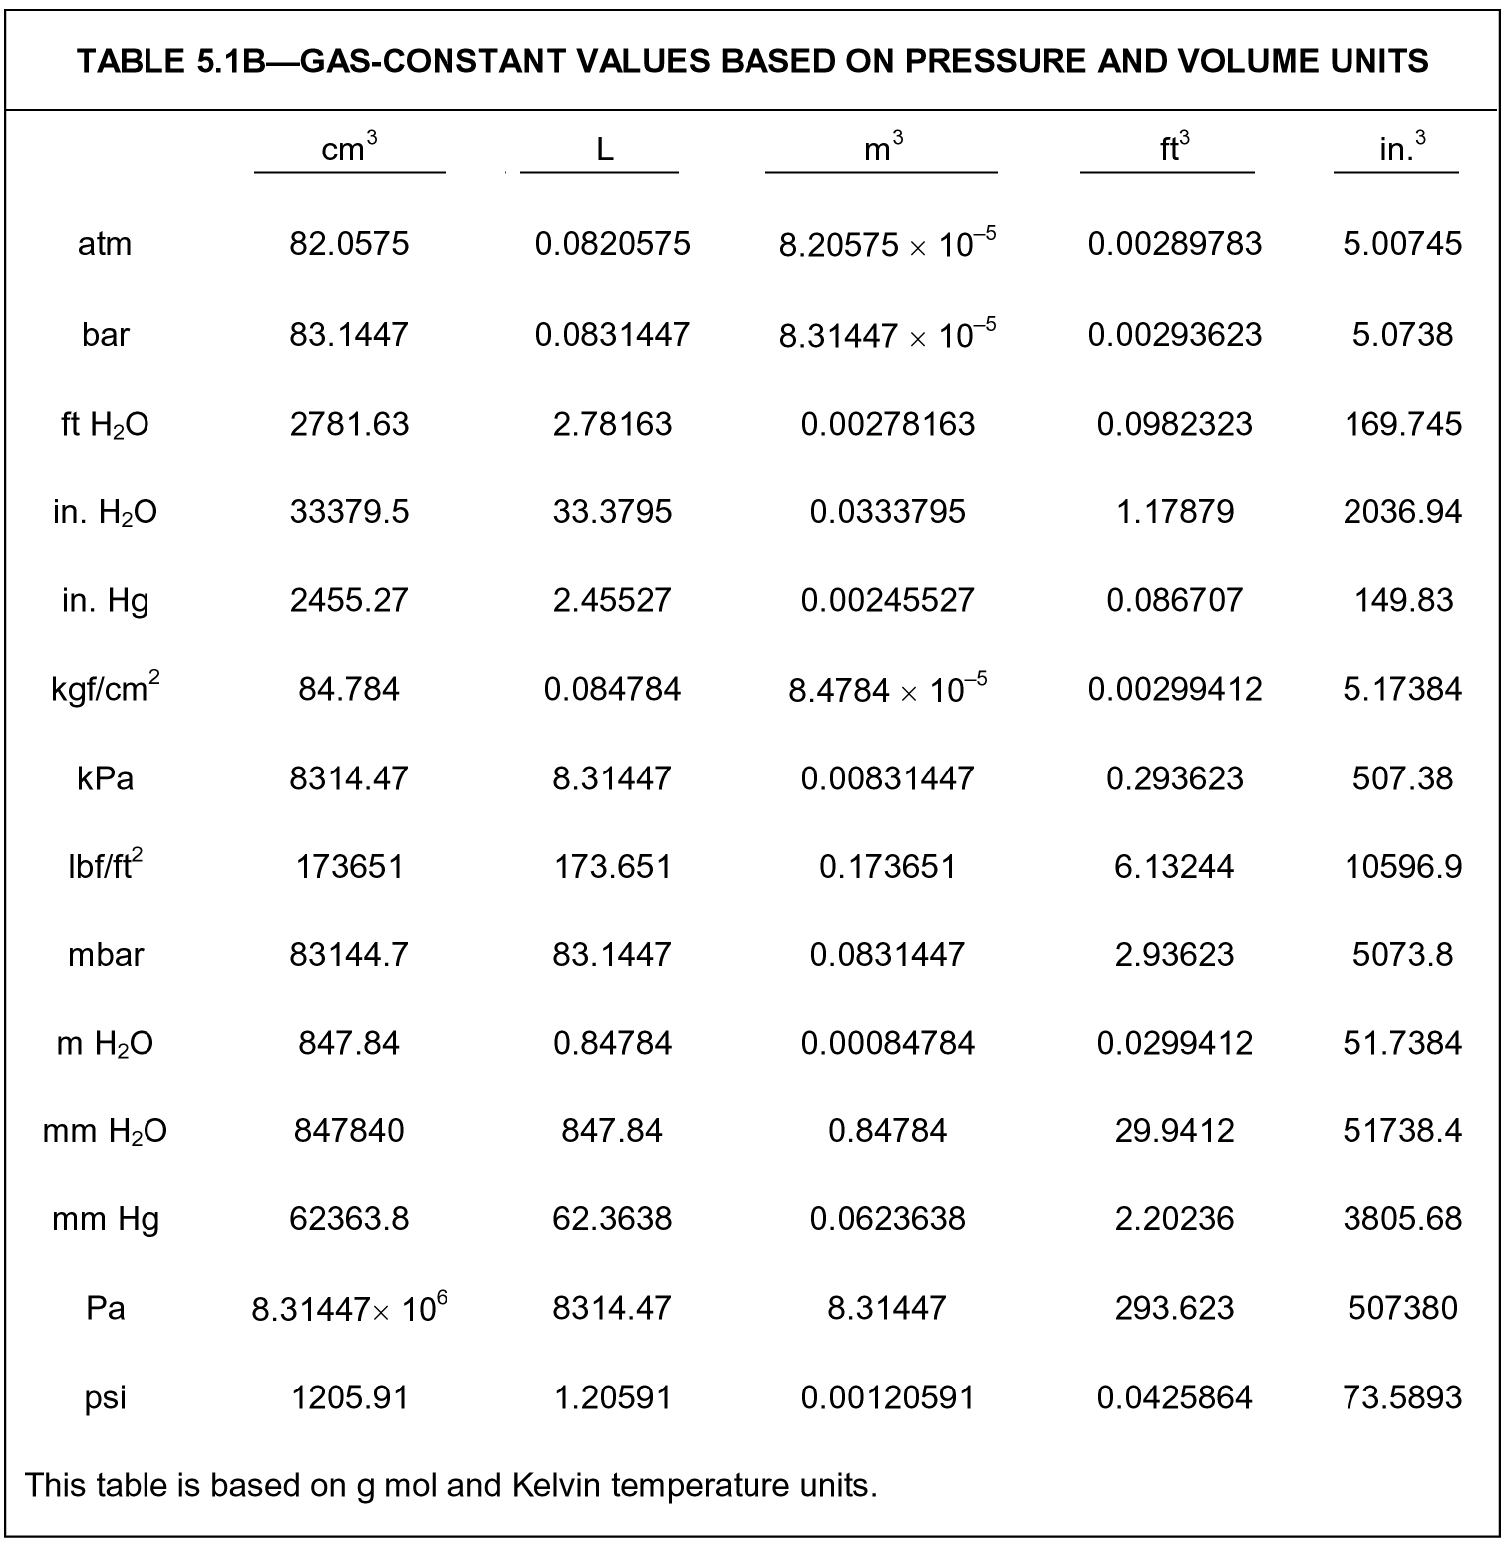
\includegraphics[scale=1]{images/Vol_2.png}
    \caption{Table 1B}
    \label{fig:figure2}
\end{figure}
\begin{figure}[!hbpt]
    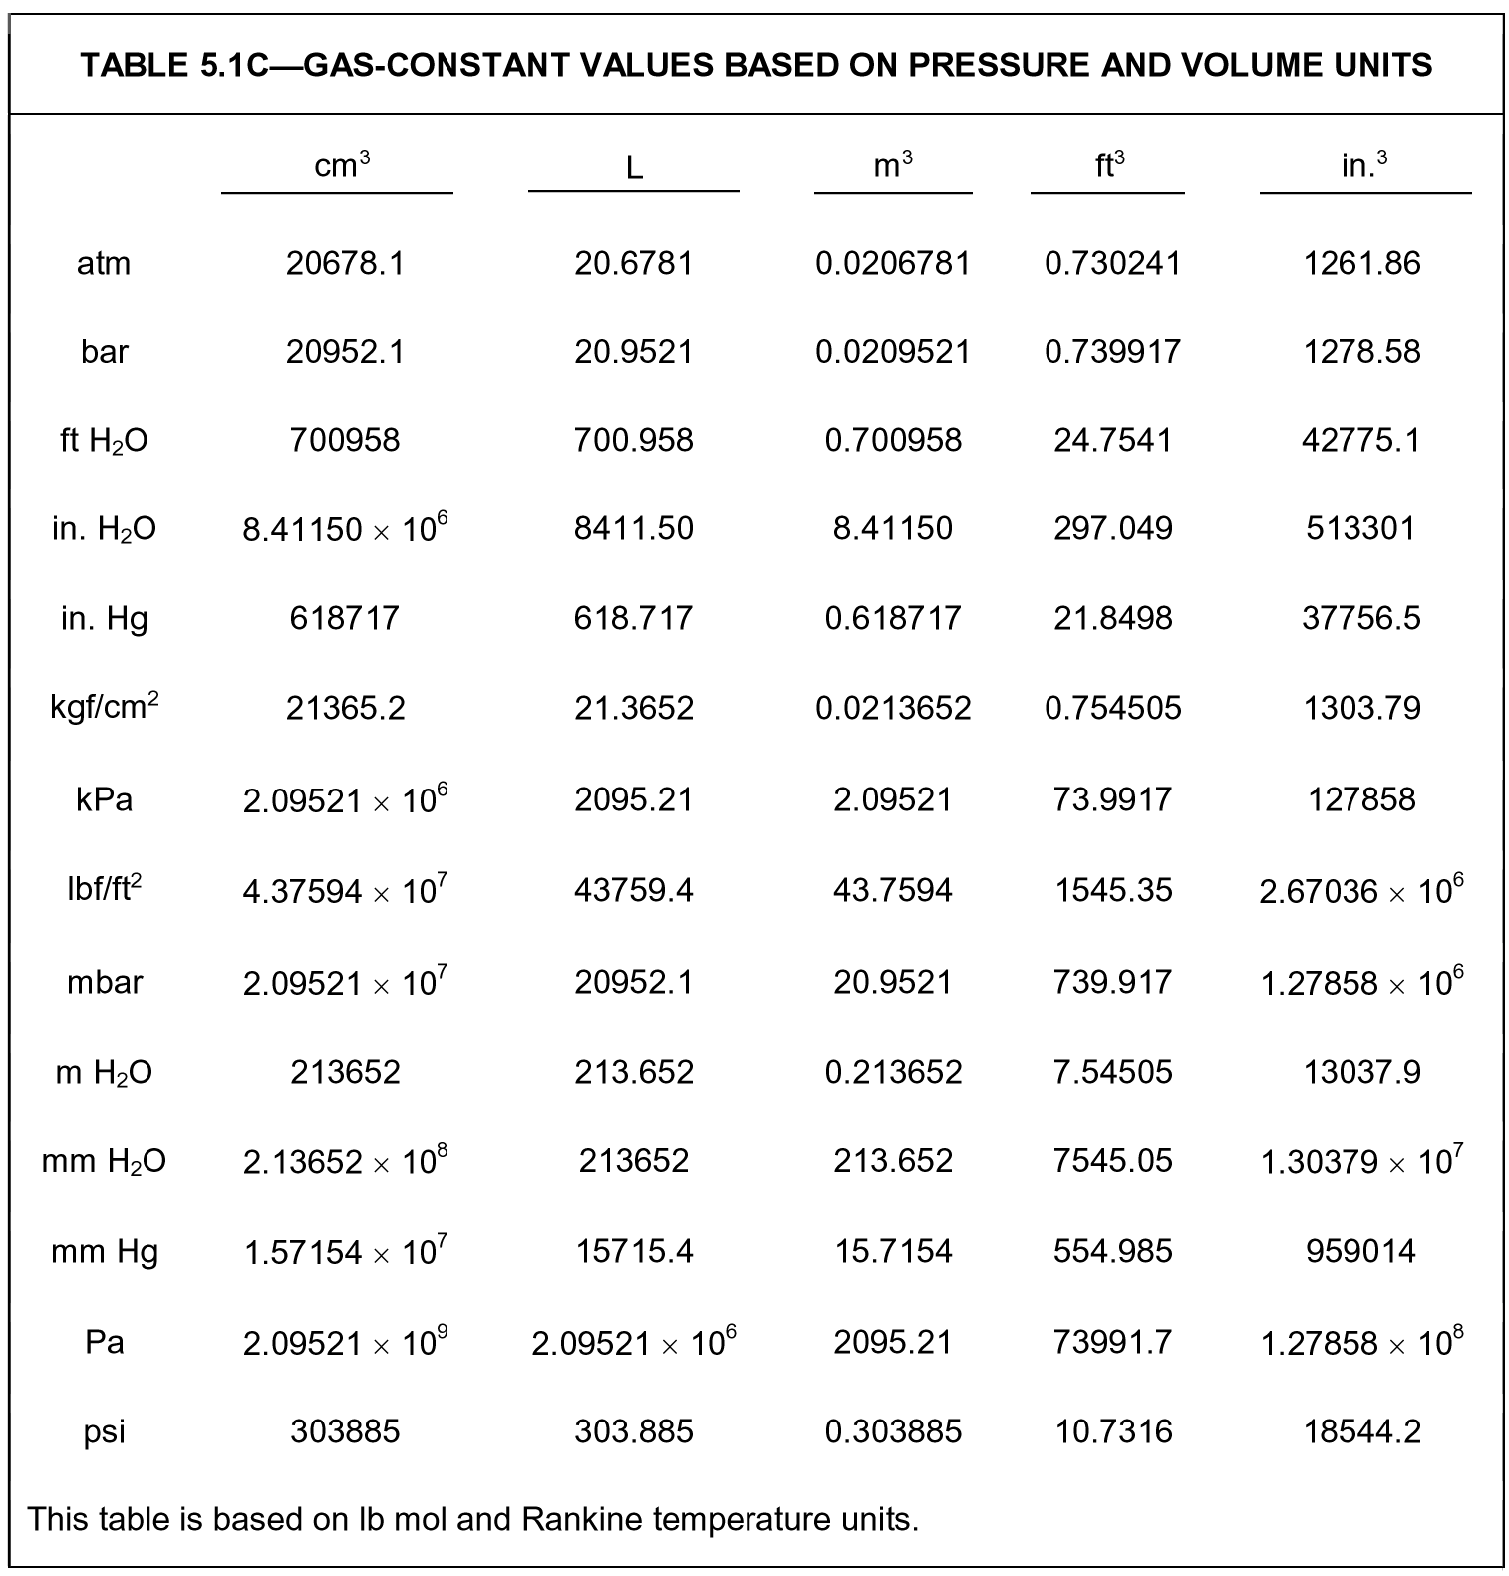
\includegraphics[scale=1]{images/Vol_3.png}
    \caption{Table 1C}
    \label{fig:figure3}
\end{figure}




\section{Ideal Gas Mixtures}
The Ideal Gas Law, i.e. eq~\ref{eq:idealgaslaw} also holds true for a system containing multiple ideal gases.
An ideal gas mixture partitions the total pressure into the partial pressure contribution of each component.


Thus, the eq~\ref{eq:idealgaslaw} can be rewritten as:
\begin{equation}
    P_{i}V = n_{i}RT
\end{equation}
where,
\begin{itemize}
    \item $P_{i}$ is Partial Pressure of the component
    \item $n_{i}$ is number of moles of the component
\end{itemize}



\section{Real gas as ideal gas}
Ideal gases is a theoretical concept but real gases behave ideally under certain conditions. Systems with very low pressures or high temperature are said to show "ideal gas" behaviour. This is because at low pressure and high temperature, inter-molecular forces between the particles is low

\section{Conclusion}
The ideal gas equation is significant because it is a tool used for making predictions, doing calculations and understanding of gas behaviour under different conditions. It is used extensively in various scientific and engineering fields, including thermodynamics, chemistry, physics and material science.

\bibliography{refs}
\bibliographystyle{plain}







\end{document}
